%% ------------------------------------------------------------------------- %%
\chapter{Lean Startup}
\label{cap:leanstartup}
\section{Lean Startup: O que é}
\subsection{Startup: uma definição}
\par Através da popularização da internet e dos computadores pessoais nos anos 90, nos Estados Unidos, o termo startup foi generalizado para classificar pequenas empresas com propostas inovadoras, sejam por atuarem com as novas tecnologias que surgiram para o grande mercado na época como as chamadas empresas online ou empresas "ponto com" ou  pelo seu novo modo de organização e processo de produção.
\par \cite{nicolo:14} provê uma definição de uma startup de software baseada nos desafios que ela enfrenta:
\begin{itemize}
\item Pouco ou nenhum histórico operacional - Startups com pouca ou nenhuma experiência em desenvolver processos de negócio e gerenciamento organizacional.
\item Recursos limitados - Startups tipicamente focam em lançar um produto, promovê-lo e construir alianças estratégicas.
\item Múltiplas Influências - Pressão dos investidores, clientes, parceiros e competidores impactam nas tomadas de decisões de uma empresa. Apesar de importantes em média elas tendem a ser inconsistentes.
\item Mercado e tecnologias dinâmicas- Empresas de softwares novas frequentemente precisam desenvolver ou operar com tecnologias disruptivas para atuar em potenciais mercados alvos.
\end{itemize}

\par Apesar de não ser um rótulo exclusivo para o mercado de Tecnologia da Informação alguns locais e atividades foram particularmente associados à classificação devido a revolução tecnológica promovida pela bolha da internet, como no Vale do Silício, área norte do estado da Califórnia, EUA, conhecida até hoje por ser um ecossistema constituído de empresas inovadoras.
\par Com o passar dos anos e com o impacto da internet no mercado global o termo amadureceu para empresa, grupo ou organização que busca um modelo de negócios escalável geralmente envolvida em implementações de processos inovadores de desenvolvimento e pesquisa de mercado-alvo.
\par Grosseiramente uma startup surge sob uma ideia ou foco que pode ou não dar certo mas consciente desta instabilidade.
\par Para Steve Blank, acadêmico e empreendedor do Vale do Silício, uma startup vai de fracasso à fracasso com objetivo de aprender com cada falha e assim definir o que não funciona no processo na qual a empresa esta engajada. Por isso é considerado um modelo de negócio escalável: deve ser flexível perante a constante reação do mercado e da própria produção.

\subsection{Lean Startup}
\par \emph{Lean Startup} (Startup Enxuta) é um conceito introduzido por Eric Ries ( \cite{ries:11}), empreendedor de diversas startups do Vale do Silício.
\par Trata-se de uma metodologia de negócios derivada da combinação de outros padrões de desenvolvimento como \emph{Minimal Viable Product} (produto viável mínimo), \emph{Customer Development} (desenvolvimento voltado ao cliente) e \emph{Agile software development} (Desenvolvimento Ágil de Software ou Método Ágil).
\par Ries propõe que é possível encurtar os ciclos de implementação de um produto (ou solução) adotando uma combinação de testes, hipóteses de negócio e degustações por parte do público-alvo. 
\par Através do lançamento periódico de cada versão do produto é possível avaliar não apenas quesitos técnicos como também a reação do mercado. 
\par Consequentemente o retorno de cada iteração afeta o planejamento do produto e suas futuras versões.
\par O retorno de cada iteração provém do Aprendizado Validado(\emph{Validated Learning}.
\par Segundo \cite{ries:11} esse modelo consiste em uma aprendizagem que possa ser validada por meio de experimentos que permitam aos empreendedoras testar cada elemento de sua visão.
\par Isso evita desperdício de desenvolvimento além de abrir oportunidades para adaptações e alterações de projeto em casos de falha ou rejeição do cliente.
\par Versões simples do produto sob cada ciclo de avaliação é uma estratégia derivada do padrão de Mínimo Produto Viável( \emph{Minimal Viable Product}), proposta em 1996 por Frank Robinson, CEO da empresa SyncDev\footnote{ Retirado de SyncDev: \url{http://www.syncdev.com/minimum-viable-product/}}, porém popularizado anos depois por Steve Blank( \cite{junk:2000}).
\par Robinson propõe o lançamento de uma versão o mais simples possível de modo à antecipar a análise de mercado e assim minimizar o risco de retorno por parte da empresa.
\par A popularidade Steve Blank foi em adaptar a estratégia incluindo o lado do cliente, o que ele chama de \emph{Customer Development}. Blank vai além de apenas minimizar o risco de retorno: busca compreender as necessidades do cliente.
\par O \emph{Lean Startup} aprimora ainda mais o conceito para avaliações sob cada iteração e assim maximizar o aprendizado e evolução do projeto alinhado com o desejo do mercado. Esse ciclo de evolução e aprendizado é chamado Construir-Medir-Aprender (\emph{Build-Measure-Learn}).

\section{Produto Mínimo Viável (MVP)}

\par Uma definição de Produto Mínimo Viável por Eric Ries (\cite{ries:11}):
\emph{"Um Produto Mínimo Viável é uma versão de um novo produto na qual permite que a equipe de desenvolvimento colete o máximo de aprendizado válido sobre o cliente com o mínimo de esforço."}.
    \par A idéia central do conceito de MVP é maximizar a validação de aprendizado sobre um produto utilizando o menor esforço possível.
    \par Como na maioria das startups os recursos financeiros e humanos são bastante escassos o tempo de validação do produto e determinação do interesse do público é um fator decisivo para o sucesso da mesma.
    \par Um MVP deve possuir 3 características \footnote{ Retirado de Techopedia: Minimum Viable Product (MVP): \url{https://www.techopedia.com/definition/27809/minimum-viable-product-mvp}}.:
    \begin{enumerate}
        \item Ter valor suficiente para que uma pessoa queira utilizá-lo ou comprá-lo.
        \item Possui suficientes benefícios para reter os chamados usuários pioneiros (emph{early adopters}) \footnote{Os primeiros consumidores de um produto que acaba de tornar-se disponível}.
        \item Ser capaz de prover um ciclo de \emph{feedback} suficiente para guiar o desenvolvimento.
\end{enumerate}
    \par Durante a concepção do projeto são definidas algumas hipóteses sobre o produto e na etapa do MVP é definido então qual será o seu núcleo, ou seja, quais funcionalidades ou estratégias deseja-se testar de modo que possam validar as hipóteses iniciais e obter o máximo de aprendizado possível utilizando-o para planejar novas funcionalidades e determinar as prioridades para a equipe de desenvolvimento.
    \par Além da validação de aprendizado outra vantagem significativa provida pelo MVP é evitar desperdícios.
    \par O MVP permite testar se a funcionalidade ou hipótese sobre um projeto é bem aceita pelo público alvo implementando-a de uma forma simplificada sem despender horas a fio de desenvolvimento.
    \par Dessa forma caso comprove-se que tal premissa não é interessante para o projeto seu desenvolvimento é interrompido sem que tenham sido desperdiçados tempo e recursos.
    \par Os termos "mínimo" e "máximo" referentes a "máximo aprendizado" e "mínimo produto viável" frequentemente se mostram vagos na documentação do que é um MVP, como o próprio Eric Ries esclarece a aplicação desse termos não é um conceito rígido e varia de acordo om o contexto e julgamento de quem estiver aplicando-o \footnote{Fonte: Startup Lessons Learned, Minimum Viable Product: a guide \url{http://www.startuplessonslearned.com/2009/08/minimum-viable-product-guide.html}}. 
    \par É importante ressaltar que um MVP não é um produto completo com as funcionalidades  mínimas e sim um conjunto de características mínimas que configuram o serviço ou produto que está sendo oferecido.
    \par Dessa forma um MVP pode ser apenas um protótipo, um produto completo ou mesmo apenas um \emph{mock-up} do que será oferecido na versão completa.
    \par Alguns tipos de MVP são: \footnote{ Fonte: Scale my Business: The Ultimate Guide to Minimum Viable Products  \url{http://scalemybusiness.com/the-ultimate-guide-to-minimum-viable-products/}}
\begin{itemize}
\item \emph{ Vídeo Explicativo:}
Um vídeo curto contendo uma explicação clara do que o seu produto faz e porque as pessoas deveriam utilizá-lo. Esse é o caso do dropbox que fez um video \footnote{Link para o vídeo  \url{https://www.youtube.com/watch?v=7QmCUDHpNzE}} com cerca de 5 minutos explicando o que era o seu serviço.
\item \emph{Landing Page:}
Criar uma página inicial contendo uma explicação detalhada do que é o produto que você irá oferecer juntamente com um formulário de contato. Através de uma configuração simples pelo Google Analytics é possível manter um registro de conversões (no caso cadastros do formulário)  a fim de medir o interesse das pessoas no seu produto.
\item \emph{MVP "Mago de OZ":}
A idéia é criar uma página visualmente completa que funcione como o produto final mas que na verdade  exista alguém  executando as tarefas manualmente. Esse foi o caso da Zappos hoje a maior vendedora de sapatos dos Estados Unidos.
\item \emph{ MVP com Consierge:}
Ao invés de prover um produto você realiza manualmente o serviço executando
exatamente os mesmos passos para o usuário que o a sua empresa realizaria. É um método não escalável e lento para executar pois requer que você esteja em contato direto com o cliente e realize as tarefas manualmente porém isso permite um rápido aprendizado sobre o produto e o cliente.
\\A empresa Food on the Table ajuda seus consumidores a criarem listas de compras, acharem receitas e conseguirem descontos nos ingredientes em seus supermercados favoritos, inicialmente seus fundadores encontraram uma senhora interessada no serviço e por 10 dólares/semana eles mantinham as listas de compra e procurava, por descontos nos supermercados em que ela fazia  compras.
\end{itemize}

\section{O ciclo de Build-Measure-Learn}

    \par Um ciclo de build measure learn é uma abordagem de desenvolvimento do produto que aprimora  o tradicional modelo de desenvolvimento "Cascata" utilizado de forma abrangente durante o século XX.
\subsection{O modelo Cascata}
    \par O nome "Cascata" é bastante literal e tem origem na própria estrutura do método (figura \ref{fig:waterfall}) que seguia uma série de passos de forma sequencial de maneira bastante direta, como se fosse uma cascata.
\begin{figure}[htb]
\centering
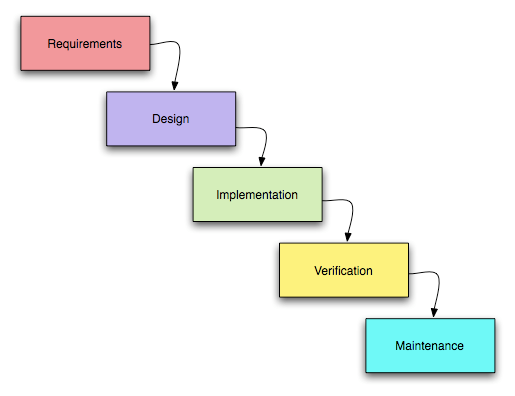
\includegraphics[width=10cm]{figuras/waterfall}
\caption{\label{fig:waterfall}O Modelo Cascata.}
\end{figure}
\par O método consiste em um desenvolvimento sequencial e não-iterativo inicializando com a parte de análise de requisitos e de forma subsequente temos as etapas de design de projeto, implementação, verificação e manutenção.

Uma rápida explicação dos passos:
\begin{itemize}
\item \emph{ Requerimentos:} Realizar a análise de requisitos do projeto.
\item \emph{ Design de Projeto:}  Focando na estrutura de dados, arquitetura do software, detalhes procedais e caracterização das interfaces é formulado um documento de forma a apresentar os requerimentos de uma forma que possa ser interpretado pelos programadores.
\item \emph{ Implementação:} Etapa da codificação do projeto propriamente dita.
\item \emph{  Verificação: } Etapa para teste do produtos visando eliminar qualquer \emph{bug} que possa ter passado despercebido e refinar a lógica interna do software caso necessário.
\item \emph{ Manutenção: } Etapa para instalação do sistema no cliente, configuração de servidores, etc.
\end{itemize}

\par Uma das grandes das críticas dessa abordagem é que dificilmente um desenvolvimento de software segue todas as etapas da forma como o modelo propõe e nem sempre o cliente sabe definir bem os requisitos antes de ver o software funcionando, resultando em tempo e desenvolvimento desperdiçado em funcionalidades que não resolvem o problema. Mudanças tardias no escopo do projeto encarecem o custo total e poderiam ter sido evitadas e contornadas de maneira mais satisfatória em um modelo com um processo de desenvolvimento iterativo \footnote{ Fonte: Wikipedia - Waterfall Model \url {https://en.wikipedia.org/wiki/Waterfall_model}}. Ao contrário do modelo cascasta no qual o contato do cliente com o software se dá apenas no fim do processo de desenvolvimento na etapa de testes o método de \emph{Build-Measure-Learn} privilegia desde o início uma iteração contínua com o cliente.

\subsection{Build-Measure-Learn (Construir-Medir-Aprender)}
\par Na fase de Verificação do modelo Cascata existia a possibilidade de disponibilizar para os clientes versões alphas ou betas do software em questão, como o foco não era obter um retorno sobre o desenvolvimento e sim verificar a existência de \emph{bugs} o usuário acabava completamente fora do processo de desenvolvimento.
\par Com o surgimento da Metodologia Ágil foi possível criar softwares de maneira interativa e envolver o cliente no processo porém devido a falta de um arcabouço para testar as hipóteses comerciais acabava-se muitas vezes por desenvolver um software com todas as funcionalidades que o cliente gostaria mas não obter um sucesso comercial.\footnote{Fonte: Por Steve Blank em \url{http://venturebeat.com/2015/05/06/build-measure-learn-doesnt-mean-throwing-things-against-the-wall-to-see-if-they-stick/}}
\par O modelo de Construir-Medir-Aprender surge então com o principal objetivo de eliminar as incertezas sobre as hipóteses do produto. Através de um aprendizado rápido sobre o comportamento dos usuários é possível minimizar os riscos e custos desnecessários que persistir em uma idéia equivocada pode causar, mantendo o aspecto interativo presente na metodologia Ágil e obtendo um aprendizado sobre o comportamento do usuário a cada iteração. Este modelo é uma das idéias fundamentais do \emph{Lean Startup} consistindo de um ciclo de 3 fases base: Construir, Medir e Aprender. Porém para melhor ilustrar o que representa cada uma das fases foi incluído na figura \ref{fig:buildmeasurelearn} outras 3 menores (\emph{ideas, data e code}).
\begin{figure}[htb]
\centering
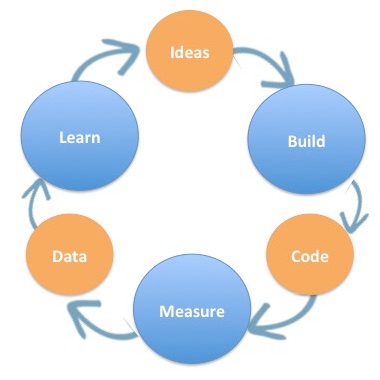
\includegraphics[width=10cm]{figuras/buildmeasurelearn}
\caption{\label{fig:buildmeasurelearn}O ciclo de Build Measure Learn.}
\end{figure}
\begin{itemize}
\item \emph{Build:} Algumas idéias são definidas a partir das hipóteses do produto que precisam ser implementadas (\emph{code}) no MVP.
\item \emph{Measure:} Implementado o MVP coleta-se os dados(\emph{data}) de uso avaliando o desempenho, ou seja, todo o ciclo é baseado na idéia de aprendizado rápido para coletar o máximo possível de informação sobre a reação dos usuários as idéias já implementadas.
\item \emph{Learn:} A partir então da análise dos dados coletados é possível inferir sobre como continuar o desenvolvimento, definir o que funcionou e o que pode ser descartado. Feito isso implementa-se as novas idéias geradas e o ciclo então é repetido para validá-las.
\end{itemize}
\par As etapas do ciclo não precisam necessariamente ocorrer em ordem podendo se sobrepor ou mesmo serem unidas dependendo de como for o ciclo de desenvolvimento(\cite{ries:11}). As alterações de software precisam ser feitas de maneira rápida de modo a testar o mais rápido possível novas idéias, portanto é importante que as funcionalidades sejam simples e diretas, pois o foco é o aprendizado gerado e não desenvolver um software ou um protótipo completo. Dessa maneira é possível evitar que sejam desperdiçados recursos no desenvolvimento de uma funcionalidade que pode não ser bem recebida.
\par Para minimizar que um sistema com problemas seja colocado em produção e acelerar o processo de desenvolvimento, procura-se utilizar ferramentas que auxiliam na integração contínua do software, além de executar testes automatizados. A utilização desses recursos permite seja possível manter um desenvolvimento consistente e confiável sem comprometer o tempo de execução.
\par O que o Construir-Medir-Aprender perde de vista é que novos empreendimentos, tanto startups quanto novas ideias dentro de empresas já existentes não começam com ideias mas com hipóteses. O conceito de "Ideia" evoca uma visão que imediatamente requer um plano para se frutificar. Em contraste, "hipótese" indica um palpite com precedentes que requer experimentação e dados para ser validado ou invalidado. (\cite{blankendeavor} ).
\par Como a construção deve estar alinhado com o as hipóteses formuladas e a cada ciclo é necessário sempre testar novas hipóteses resultando em diferentes protótipos, a figura \ref{fig:hypotheses-experiment} representa uma variação do ciclo de Construir-Medir-Aprender cuja proposta é enfatizar quais hipóteses devem ser testadas.
\begin{figure}[htb]
\centering
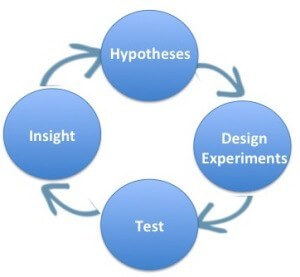
\includegraphics[width=5cm]{figuras/hypotheses-experiment}
\caption{\label{fig:hypotheses-experiment} Uma variação para o ciclo de Construir-Medir-Aprender.}
\end{figure}

\section{Desenvolvimento de Clientes}
\par Steven Blank em seu livro os 4 passos para a epifania (\cite{blank:03}) explica que o modelo de Desenvolvimento de Clientes não é um substituto para o modelo de Desenvolvimento de Produto e que na verdade ambos devem ser executados em paralelo.
\par No mesmo livro ele define o modelo de Desenvolvimento de Clientes de uma startup através da premissa: “ Aprender e descobrir quem são os clientes iniciais de uma empresa, e em quais mercados eles estão, requer um processo separado e distinto do Desenvolvimento de Produtos. A soma dessas atividades é o Desenvolvimento de Clientes.”
\par O Desenvolvimento de Clientes foca em endenter os problemas dos clientes e suas necessidades para encontrar o melhor encaixe de mercado.
\par É um processo interativo que parte da premissa de que “os fatos estão fora do escritório, dentro dele só existem opiniões” e que portanto o empreendedor deve buscar o quanto antes validar suas hipóteses fundamentais do mercado.\footnote{Manual da Startup Fonte: \url{http://www.manualdastartup.com.br/blog/customer-development-o-processo-para-se-chegar-ao-productmarket-fit/}}.
\par O processo é dividido em 4 passos (figura \ref{fig:customerdevelopment}) sendo que os dois primeiros acontecem antes do ajuste do produto ao mercado, com foco no aprendizado e validação de hipóteses, enquanto os outros dois tem foco no crescimento e otimizações.
\begin{figure}[htb]
\centering
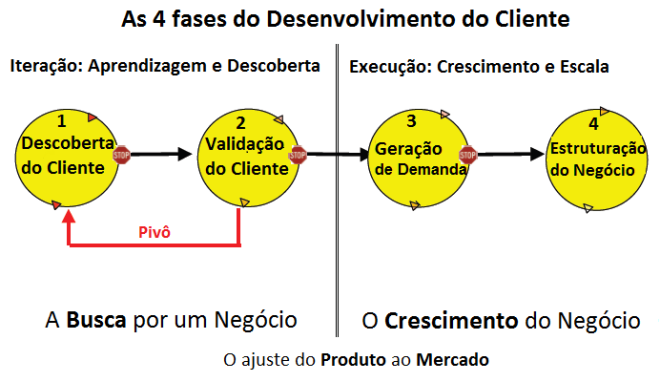
\includegraphics[width=15cm]{figuras/customerdevelopment}
\caption{\label{fig:customerdevelopment}Os 4 passos do ciclo de Customer Development.}
\end{figure}
\par A primeira fase do ciclo é compreendida pelos dois primeiros passos: Descoberta do Cliente e Validação do Cliente.
\par A segunda fase Geração de Demanda e Estruturação do Negócio é a fase para Crescimento do Negócio na qual o foco passa a ser a execução.
\par Depois de achar o encaixe de mercado é a fase na qual o objetivo está em escalar o crescimento da empresa.
\par A maior contribuição do livro Os 4 passos da epifania \cite{blank:03} está nas práticas oferecidas nos dois passos iniciais.
\par No passo de Descobrimento do Cliente o objetivo é provar que existe um problema a ser solucionado em um mercado grande o suficiente e que o seu produto supra essa necessidade.
\par Para isso é proposto sempre estar em contato com o Cliente, realizando entrevistas de modo a obter um conjunto mínimo de funcionalidades e testá-las em um MVP.
\par Já na fase de Validação do Cliente o foco é provar que existe uma maneira rentável de se adquirir e manter consumidores.
\par Na validação do Cliente é ainda é necessário descobrir se de fato existem clientes dispostos a pagar pelo seu produto e se o mesmo provoca uma mudança na rotina do usuário.
